\documentclass{beamer}

\usepackage[utf8]{inputenc}
\graphicspath{{../Graphics/}}

%Information to be included in the title page:
\title{Heat Energy Sources in Canada}
\author{Noah Bolohan, Anton Iatcenko, Ryan Thiessen, Yakine Bahri, Benjamin MacAdam, Alireza Yazdani}
\institute{Math\textsuperscript{Industry}}

\date{August 2020  \\ \vspace{30pt} 
\includegraphics[scale=0.3]{pims_logo.png} }



\begin{document}

\frame{\titlepage}

\begin{frame}
\frametitle{The Data Set}
what the data is, where it came from
\end{frame}


\begin{frame}
\frametitle{The Big Picure}
Canada as a whole (pie chart)
\end{frame}


\begin{frame}
\frametitle{Change Over Time I}
stacked bars (4 per slide)
\end{frame}


\begin{frame}
\frametitle{Change Over Time II}
stacked bars (4 per slide)
\end{frame}


\begin{frame}
\frametitle{Change Over Time III}
stacked bars (4 per slide)
\end{frame}


\begin{frame}
\frametitle{Province Groupings}
stacked bars (all together)
\end{frame}


\begin{frame}

\frametitle{Cause of the Groupings: Natural Gas}
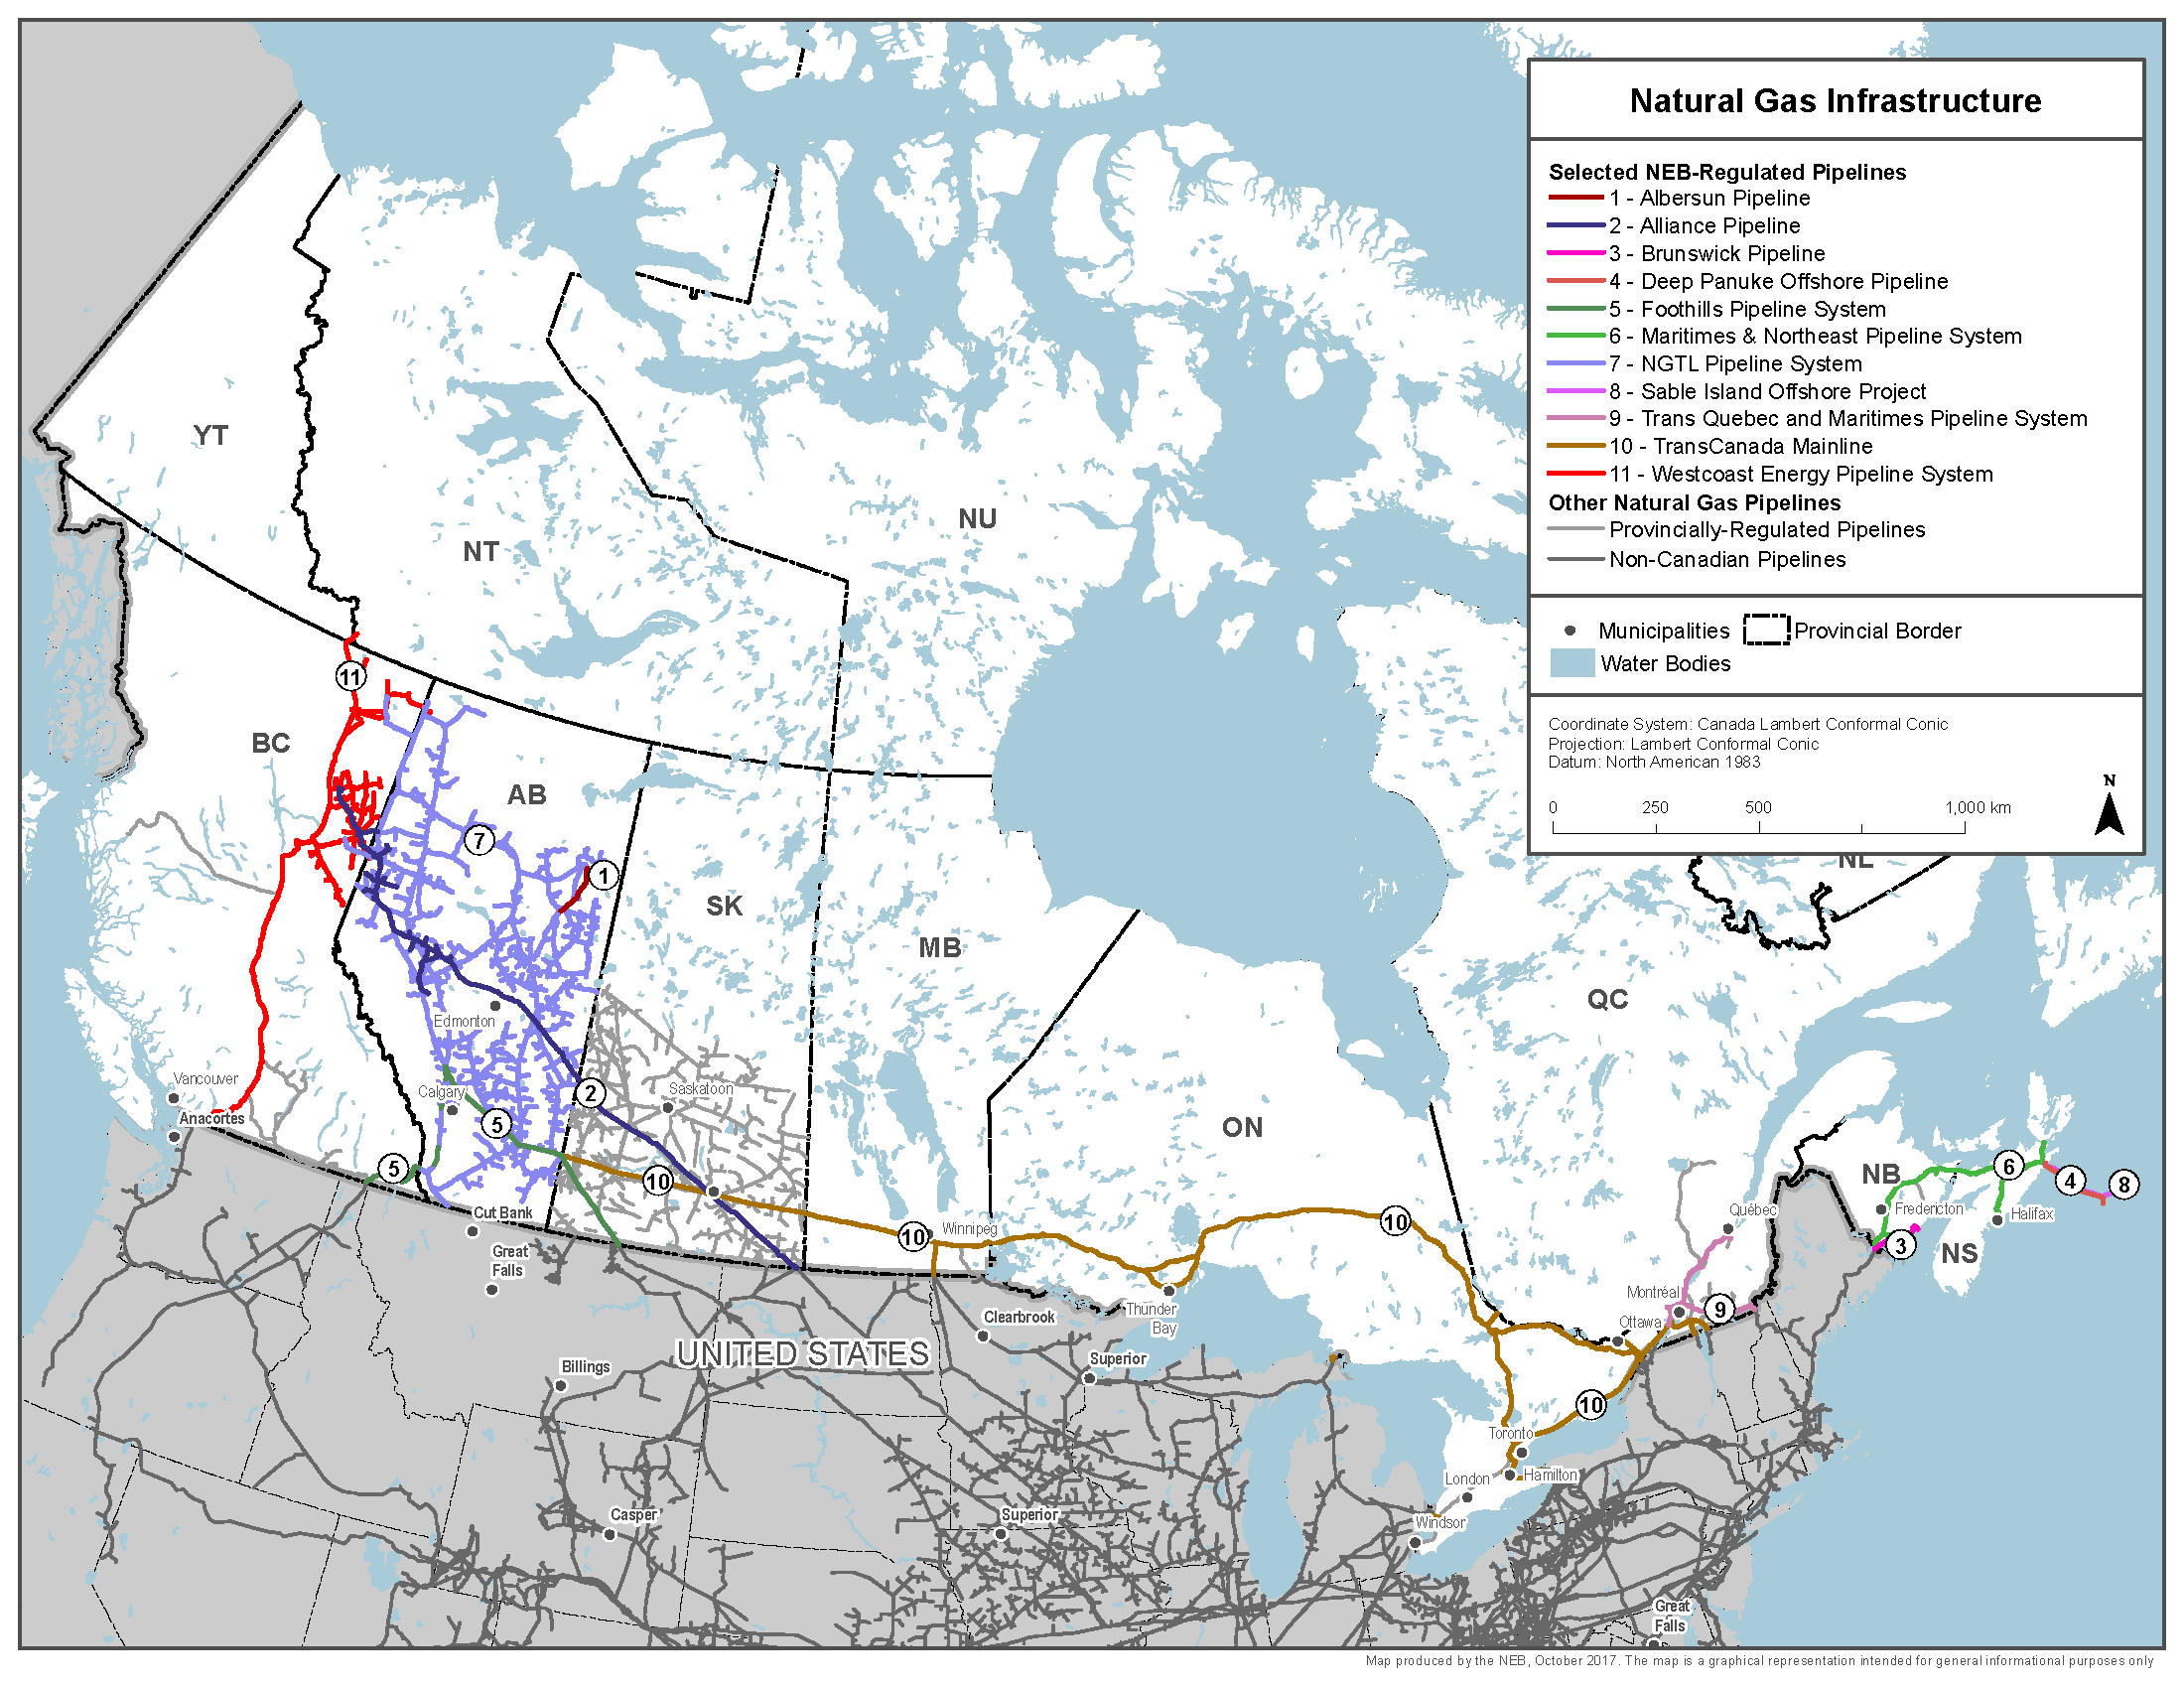
\includegraphics[width=0.6\textwidth]{natural_gas_pipeline_natural_resources_canada}
\small
\begin{itemize}
	\item Saskatchewan, Alberta, and parts of British Columbia have an extensive natural gas infrastructure, giving those provinces affordable, easy access to a relatively clean power source for heating.
	\item Although Manitoba and Ontario do not have much natural gas infrastructure, the significant population centers Winnipeg and Toronto have access to the TransCanada pipeline, making those regions heat source of choice to be natural gas.
\end{itemize}
\normalsize
\end{frame}


\begin{frame}
\frametitle{Cause of the Groupings: Electricity}

\end{frame}


\begin{frame}
\frametitle{Cause of the Groupings: Atlantic Provinces}

\end{frame}



\begin{frame}
\frametitle{Summary}

No change over time. 

The dependence is predominantly geographic. 

Thanks for your attention.  

\end{frame}













\end{document}



















